%================================================================
%                           N O T E S
%                           ---------
%
%                           ---------
%-----------------------------------------------------------------
%                       INTRODUCTION
%-----------------------------------------------------------------
\section{Introduction}
We now want to consider what happens inside a cylinder of different density to the outside medium. We consider our same plane wave inciding on this cylinder see \figref{fig:problem_2}. The goal in this section is to find an expression for the velocity field inside the cylinder, combine this with our result in Chapter \ref{chp:outside} to plot the complete field over the entire domain. \par
%
This is referred to as a \emph{transmission problem} in the literature, see for example \cite[$\S$1.3.3]{martin06scattering} since the wave is not bounded at the cylinder walls but transmitted through. \par
%
The statement of the problem is as follows. We are given an incident field, $\Phiin$ for which we need to find the field at the cylinder wall, $\Phi_{r=\sigma}$ and the field inside the cylinder wall $\Phi_{r<\sigma}$.
%
  \begin{figure} \centering
    %
    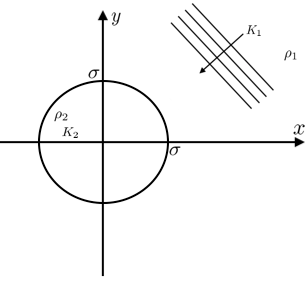
\includegraphics[width=6cm]{../figures/prob2_sketch.png}
    %
    \caption{The transmission problem}\label{fig:problem_2}
    %
  \end{figure}
%
The velocity field inside the cylinder will be subject to the same physics as the one outside the cylinder. We can therefore find the scattered field inside the cylinder in the same way we found the scattered field outside the cylinder in section \ref{ss:scattered_field}. \par
%
  \begin{equation}
    \Phi_{\text{inside}} = \sum^\infty_{n=0} \epsilon_n i^n \hat{A} \text{ Bessel}(kr) \cos(n(\theta-\alpha))
  \end{equation}
  \begin{equation}
    \Phi_{\text{outside}} = \sum^\infty_{n=0} \epsilon_n i^n \hat{B} H(kr) \cos(n(\theta-\alpha))
  \end{equation}
%
In \ref{ss:scattered_field} we made our choice of cylindrical function to be used by describing the far field, and realising it must satisfy the Sommerfeld Radiation Condition (definition \ref{defn:sommerfeld_radiation_condition}). In the same way here we consider the field as we approach the origin. Outside the cylinder the Bessel function must still be of the third kind since it must still satisfy the Sommerfeld Radiation Condition.
%
%---------------------------------------------------------------------
%
%               BESSEL FUNCTIONS APPLIED TO THIS PROBLEM
%
%---------------------------------------------------------------------
\section{Bessel functions applied to this problem}
These propositions will become useful later in the chapter.
%
  \begin{propn}\label{propn:bessel_at_origin}
    Bessel functions of the first kind of integer order are well defined at the origin. In particular,
    \begin{align}\label{propn:bessel_arg_zero}
        J_n(0) =\left\{
          \begin{array}{c l}
               1 & n = 0 \\
               0 & n \neq 0
          \end{array}\right.
    \end{align}
  \end{propn}
  %              PROOF
  \begin{proof}
    This is immediate from the definiton of Bessel functions (definition \ref{defn:bessel_func}).
      \begin{align*}
        J_n(x)
          &= \sum^\infty_{m=0} \frac{(-1)^m(x/2)^{n+2m}}{m! (n+m)!}\\
          &= \frac{(-1)^0(x/2)^{n}}{0!n!}         %m=0
            + \frac{(-1)^1(x/2)^{n+2}}{1!(n+1)!}  %m=1
            + \frac{(-1)^2(x/2)^{n+4}}{2!(n+2)!}  %m=2
            + \dotsb \\
          &= \left(\frac{x}{2}\right)^n
            \left[\frac{1}{n!}           %m=0
            - \frac{(x/2)^{2}}{(n+1)!}   %m=1
            + \frac{(x/2)^{4}}{2(n+2)!}  %m=2
            + \dotsb \right]\\
        \therefore
        J_0(x)
          &= 1
            - \frac{(x/2)^{2}}{2}
            + \frac{(x/2)^{4}}{12} + \dotsb
      \end{align*}
    Hence the function is well defined at $x=0$, and \ref{propn:bessel_arg_zero} holds for all $n \in \bb{Z}$.
  \end{proof}\par
%
\begin{figure} \centering
  %
  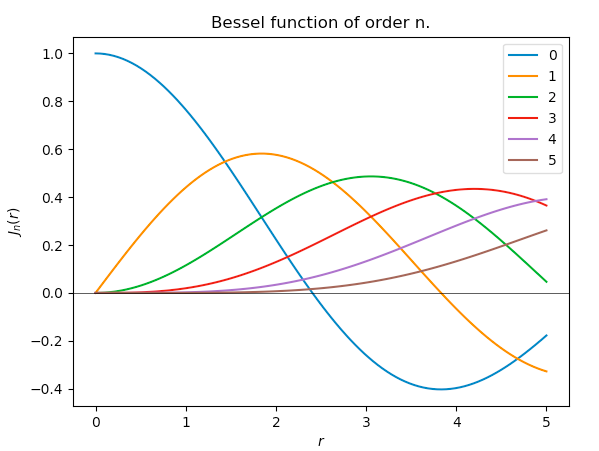
\includegraphics[width=8cm]{../figures/plot_bessel_int_order}
  \caption{Bessel functions of integer order.}\label{fig:bessel_int_problem}
  %
\end{figure}\par
%
This result is clearly shown in \figref{fig:bessel_int_problem}.
%
  \begin{propn}\label{propn:neumann_singular_at_origin}
    Neumann functions are singular at the origin.
  \end{propn}
  %
  \begin{proof}
    From the definition of Neumann functions (definition \ref{defn:neumann_func}) we know that for $n$ integer
      \begin{equation}
        Y_n(z=0) = \lim_{\nu \rightarrow n} \frac{J_\nu(0) \cos (\nu \pi) - J_{-\nu}(0)}{\sin (\nu \pi)}
      \end{equation}
    %
    First, consider the limit of the numerator as $\nu \rightarrow$ integer. Then
    %
      \begin{gather*}
        J_\nu(0) \rightarrow
          J_n(0) = \left\{
            \begin{array}{c l}
                 1 & n = 0 \\
                 0 & n \neq 0
            \end{array}\right. \text{ from proposition \ref{propn:bessel_at_origin},}\\
        J_{-\nu}(0) \rightarrow
          (-1)^nJ_n(0) = (-1)^n\left\{
            \begin{array}{c l}
                 1 & n = 0 \\
                 0 & n \neq 0
            \end{array}\right.
            = \left\{
              \begin{array}{c l}
                   1 & n = 0 \\
                   0 & n \neq 0
              \end{array}\right. \text{ from proposition \ref{propn:bessel_int_order_identity}.}\\
        \text{Hence } J_{\pm\nu}(0) \rightarrow
          \left\{
            \begin{array}{c l}
                 1 & n = 0 \\
                 0 & n \neq 0
            \end{array}\right.
      \end{gather*}
    Additionally,
      \begin{gather*}
        \cos(\nu\pi) \rightarrow (-1)^n.
      \end{gather*}
    We broady have two cases for the numerator, $n=0$ and $n\neq 0$.
      \begin{gather*}
        J_\nu(0)\cos(\nu\pi) - J_\nu(0) \rightarrow
        \left\{
          \begin{array}{c l}
               1\times1-1=0 & n = 0 \\
               0\times1-0=0 & n \neq 0
          \end{array}\right.
      \end{gather*}
    Now for the denominatory, clearly
      \begin{gather*}
        \sin(\nu\pi) \rightarrow 0.
      \end{gather*}
    This gives us the indeterminate limit $0/0$ at $x=0$ as $\nu \rightarrow$ integer.
  \end{proof}
%
\begin{figure} \centering
  %
  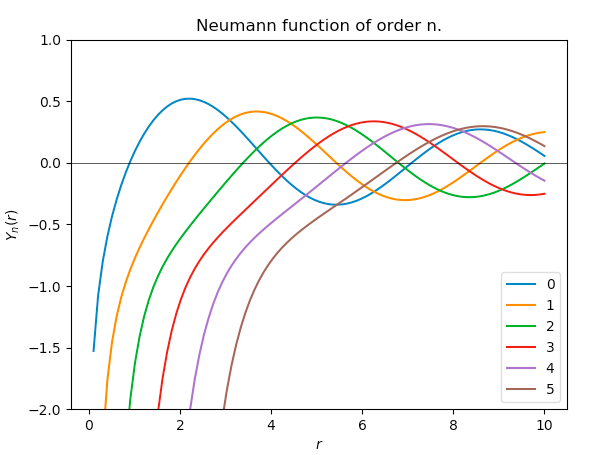
\includegraphics[width=8cm]{../figures/plot_neumann_int_order}
  \caption{Neumann functions of integer order.}\label{fig:neumann_int_problem}
  %
\end{figure}\par
%
\begin{propn}
  Hankel functions are singular at the origin.
\end{propn}
%
\begin{proof}
  This follows directly from the definition of Hankel functions for $n\in\bb{Z}$ (definition \ref{defn:hankel_func}), and can be proven in the same way as proposition \ref{propn:neumann_singular_at_origin}.
\end{proof}
%
\begin{figure} \centering
  %
  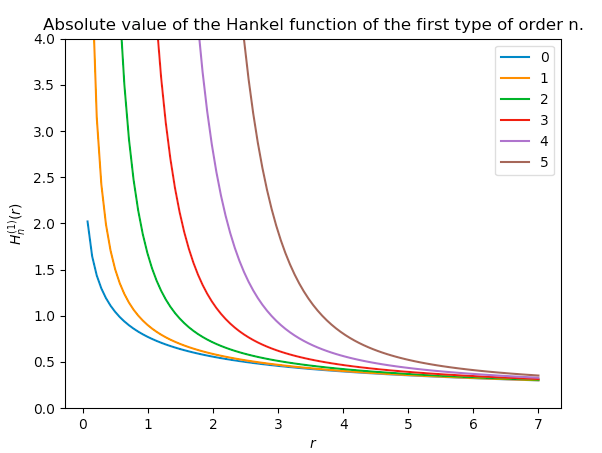
\includegraphics[width=8cm]{../figures/plot_hankel_int_order}
  \caption{Hankel functions of integer order.}\label{fig:neumann_int_problem}
  %
\end{figure}\par
%---------------------------------------------------------------------
%
%                 BOUNDARY CONDTIONS
%
%---------------------------------------------------------------------
\section{Boundary conditions}
The complete velocity field must be
  \begin{enumerate}
    \item continuous at the boundary,
    \item well defined as $r \rightarrow \infty$,
    \item and well defined as $r \rightarrow 0$.
  \end{enumerate}\par
%
These conditions will be sufficient to find an expression for the total field, which as before will be defined as
  \begin{equation}
    \PPhi{tot} = \PPhi{in} + \PPhi{out}.
  \end{equation}\par
%
Condition 1 will be satisfied by our choice of Bessel function. From the previous section we know that only Bessel functions are well defined for at the origin for integer $n$, so the $r$ dependence for our solution can be a Bessel function only.
%
Condition 2 is immediatelly satisfied by our solution to the first problem, since that solution was chosen to satisfy the Sommerfeld Radiation Condition. \par
%
We can restate Condition 3 as follows.
  \begin{equation}\label{eq:in_boundary_conditon}
    \partialfrac{\PPhi{out}}{r}\bigg\vert_{r=\sigma} =  \partialfrac{\PPhi{in}}{r}\bigg\vert_{r=\sigma}.
  \end{equation}\par
%
